%!TEX TS-program = lualatex

\documentclass[t]{beamer}
\usefonttheme[onlymath]{serif}
% For 16:9 aspect ratio:
% \documentclass[aspectratio=169,t]{beamer}

%%% Preamble
\usetheme{ThesisSlides} % Theme

%%% Font setup
\usepackage{fontspec}

\defaultfontfeatures{Ligatures=TeX}
\setmainfont{Times New Roman}
\setmonofont{FreeMono}

%%% Beamer theorem environments
\newtheorem{rtheorem}{Theorem}
\newtheorem{rproof}{Proof}
\newtheorem{rexample}{Example}

%%% Math packages
\usepackage{mathtools} % Loads amsmath automatically
\usepackage{amsfonts,amssymb,amsthm}
%%% Custom commands
\DeclareMathOperator{\sgn}{\mathop{sgn}}

%%% Sign transfer in formulas
\newcommand*{\hm}[1]{#1\nobreak\discretionary{}
{\hbox{$\mathsurround=0pt #1$}}{}}

%%% Graphics
\usepackage{graphicx}
\graphicspath{{../images/}}
\setlength\fboxsep{3pt}
\setlength\fboxrule{1pt}

%%% Tables
\usepackage{array,tabularx,tabulary,booktabs}
\usepackage{longtable}
\usepackage{multirow}

%%% Other packages
\usepackage{csquotes}
\usepackage{multicol}

%%% Drawing
\usepackage{tikz,calc,ifthen,color}
\usetikzlibrary{arrows.meta, positioning, shapes.geometric}

\title{Your Thesis Title}
\subtitle{Thesis defense}
\author{Author: Your Name \\
\vspace{0.7\baselineskip}
Advisor: Prof.\ Your Advisor}
\institute{Your University \\
Your Department}
\date{\the\year}

\begin{document}
%%% Slide content

\frame[plain]{\titlepage} % Title slide

%-------------------------------------------------------------------------------

\section{Goals and objectives}

\begin{frame}
\frametitle{\insertsection}

\textbf{Goal:} improve the effectiveness of the proposed approach in the target domain

\vspace{\baselineskip}

\textbf{Objectives:}
\begin{itemize}
    \item review existing approaches and identify limitations
    \item analyze requirements and constraints
    \item design and implement a prototype system
    \item evaluate through experimental research
    \item compare results with existing alternatives
\end{itemize}
\end{frame}

%-------------------------------------------------------------------------------

\section{Input and output data}

\begin{frame}
\frametitle{\insertsection}

\textbf{Input data:}
\begin{itemize}
    \item dataset of sample measurements
    \item configuration parameters
    \item baseline metrics from existing solutions
\end{itemize}

\vspace{\baselineskip}

\textbf{Output data:}
\begin{itemize}
    \item prototype implementation
    \item experimental results
    \item comparative analysis report
\end{itemize}
\end{frame}

%-------------------------------------------------------------------------------

\section{System analysis results}

\begin{frame}
\frametitle{\insertsection}

\textbf{Functions:}
\begin{itemize}
    \item data ingestion and preprocessing
    \item analysis and transformation
    \item result generation and visualization
    \item logging and monitoring
    \item reporting and export
\end{itemize}

\vspace{\baselineskip}

\textbf{Subsystems:}
\begin{itemize}
    \item data processing subsystem
    \item analysis engine subsystem
    \item user interface subsystem
    \item monitoring and logging subsystem
\end{itemize}
\end{frame}

%-------------------------------------------------------------------------------

\section{Design evaluation}

\begin{frame}
\frametitle{\insertsection}

\textbf{Goal:} select the optimal architecture

Criteria: performance, accuracy, scalability, maintainability

\vspace{\baselineskip}

\begin{tabular}{|l|c|c|c|}
\hline \textbf{Alternative} & \textbf{Score} \\
\hline Monolithic      & 7.15 \\
\hline Microservices    & 7.95 \\
\hline \textbf{Hybrid} & \textbf{8.30} \\
\hline
\end{tabular}

\vspace{\baselineskip}

Selected approach: \textbf{Hybrid architecture}
\end{frame}

%-------------------------------------------------------------------------------

\section{System architecture}

\begin{frame}
\frametitle{\insertsection}

\begin{figure}
    \center
    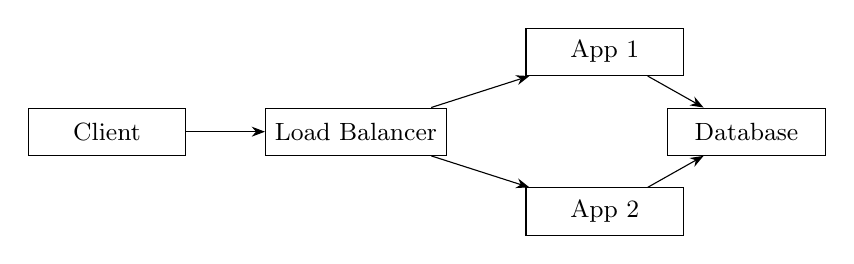
\begin{tikzpicture}[scale=0.85,
        box/.style={rectangle, draw, minimum width=2cm, minimum height=0.6cm, align=center, font=\small},
        >=Stealth
    ]
        \node[box] (client) {Client};
        \node[box, right=1cm of client] (lb) {Load Balancer};
        \node[box, above right=0.4cm and 1cm of lb] (app1) {App 1};
        \node[box, below right=0.4cm and 1cm of lb] (app2) {App 2};
        \node[box, right=2.8cm of lb] (db) {Database};
        \draw[->] (client) -- (lb);
        \draw[->] (lb) -- (app1);
        \draw[->] (lb) -- (app2);
        \draw[->] (app1) -- (db);
        \draw[->] (app2) -- (db);
    \end{tikzpicture}
\end{figure}
\end{frame}

%-------------------------------------------------------------------------------

\section{Experimental results}

\begin{frame}
\frametitle{\insertsection}
\framesubtitle{Performance comparison}

\begin{table}[H]
  \begin{tabular}{|l|c|c|c|}
  \hline \textbf{Method} & \textbf{Small} & \textbf{Medium} & \textbf{Large} \\
  \hline Baseline A       & 0.8 s & 45.2 s & 512.0 s \\
  \hline Baseline B       & 0.5 s & 38.7 s & 478.3 s \\
  \hline \textbf{Proposed} & \textbf{0.3 s} & \textbf{22.1 s} & \textbf{287.5 s} \\
  \hline
  \end{tabular}
\end{table}

\vspace{\baselineskip}

\textbf{37--44\% improvement} over baselines
\end{frame}

%-------------------------------------------------------------------------------

\section{Key formulas}

\begin{frame}
\frametitle{\insertsection}
\framesubtitle{Mathematical foundations}

\textbf{Weighted effectiveness:}
$$E = \sum_{i=1}^{n} w_i \cdot f(x_i)$$

\vspace{0.5\baselineskip}

\textbf{Classification accuracy:}
$$\text{Accuracy} = \frac{TP + TN}{TP + TN + FP + FN} \times 100\%$$

\vspace{0.5\baselineskip}

\textbf{Scalability model:}
$$T(n) = a \cdot n + b, \quad a = 2.87 \times 10^{-4}$$
\end{frame}

%-------------------------------------------------------------------------------

\section{Architecture diagram}

\begin{frame}
\frametitle{\insertsection}
\framesubtitle{State machine of the processing pipeline}

\begin{figure}
    \centering
    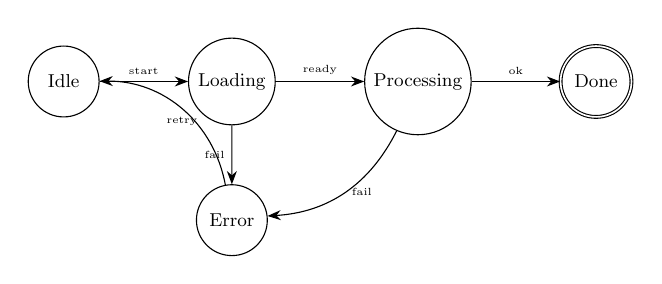
\begin{tikzpicture}[scale=0.75, transform shape,
        state/.style={circle, draw, minimum size=1.2cm, align=center, font=\small},
        accept/.style={state, double},
        >=Stealth, auto
    ]
        \node[state] (idle) {Idle};
        \node[state, right=1.5cm of idle] (load) {Loading};
        \node[state, right=1.5cm of load] (proc) {Processing};
        \node[accept, right=1.5cm of proc] (done) {Done};
        \node[state, below=1cm of load] (err) {Error};

        \draw[->] (idle) edge node {\tiny start} (load);
        \draw[->] (load) edge node {\tiny ready} (proc);
        \draw[->] (proc) edge node {\tiny ok} (done);
        \draw[->] (load) edge node[left] {\tiny fail} (err);
        \draw[->] (proc) edge[bend left] node[right] {\tiny fail} (err);
        \draw[->] (err) edge[bend right=40] node[below] {\tiny retry} (idle);
    \end{tikzpicture}
\end{figure}
\end{frame}

%-------------------------------------------------------------------------------

\section{Results}

\begin{frame}
\frametitle{\insertsection}

\begin{itemize}
    \item comprehensive literature review completed
    \item system analysis with 5 functions and 4 subsystems
    \item comparative design evaluation (hybrid approach selected)
    \item prototype implemented in Python + PostgreSQL + Docker
    \item 37--44\% performance improvement demonstrated
    \item 94.2\% accuracy achieved
\end{itemize}
\end{frame}

%-------------------------------------------------------------------------------

\section{Conclusion}

\begin{frame}
\frametitle{\insertsection}

\begin{itemize}
    \item analyzed existing approaches and identified key limitations
    \item designed modular architecture with clear subsystem boundaries
    \item implemented working prototype with comprehensive test coverage
    \item demonstrated significant improvements in performance and accuracy
    \item proposed directions for future work
\end{itemize}
\end{frame}

%-------------------------------------------------------------------------------

\end{document}
